\section{奇异同调论的公理}
\sourcepage{195}
现在引入相对奇异同调群。本节及下一节将证明，它们在所有拓扑空间偶构成的类上满足 Eilenberg--Steenrod 公理。

若 $A$ 是拓扑空间 $X$ 的子空间，则有自然的包含映射 $S_p(A)\to S_p(X)$。定义\textbf{相对奇异链群}
\[
S_p(X,A)=S_p(X)/S_p(A).
\]
边缘算子 $S_p(X)\to S_{p-1}(X)$ 在 $S_p(A)$ 上的限制正是该子空间的边缘算子，故诱导相对链上的边缘算子
\[
\partial:S_p(X,A)\to S_{p-1}(X,A).
\]
这些群和同态组成\textbf{空间偶 $(X,A)$ 的奇异链复形}，记作 $\mathcal S(X,A)$。其同调群称为\textbf{空间偶 $(X,A)$ 的奇异同调群}，记作 $H_p(X,A)$。

链复形 $\mathcal S(X,A)$ 是自由的：$S_p(X,A)$ 的一组基由所有形如 $T+S_p(A)$ 的陪集组成，其中 $T$ 是像不完全包含于 $A$ 的奇异 $p$ 维单形。

若 $f:(X,A)\to(Y,B)$ 连续，则 $f_\#:S_p(X)\to S_p(Y)$ 将 $A$ 中的链映为 $B$ 中的链，故诱导同态
\[
f_\#:S_p(X,A)\to S_p(Y,B).
\]
它与 $\partial$ 可交换，进而诱导 $f_*:H_p(X,A)\to H_p(Y,B)$。下面的结论是直接的。

\entry{定理}{4.3.1}若 $i:(X,A)\to(X,A)$ 是恒等映射，则 $i_*:H_p(X,A)\to H_p(X,A)$ 是恒等同态。若 $h:(X,A)\to(Y,B)$、$k:(Y,B)\to(Z,C)$ 连续，则 $(k\circ h)_*=k_*\circ h_*$。\translatornote{原书第一句中的同调群漏印了相对子空间 $A$。}

\sourcepage{196}
\entry{定理}{4.3.2}对 $A\subset X$ 及每个 $p$，存在同态 $\partial_*:H_p(X,A)\to H_{p-1}(A)$，使序列
\[
\cdots\longrightarrow H_p(A)\xrightarrow{i_*}H_p(X)\xrightarrow{\pi_*}H_p(X,A)\xrightarrow{\partial_*}H_{p-1}(A)\longrightarrow\cdots
\]
正合，其中 $i$、$\pi$ 均为包含映射。若 $A\ne\varnothing$，对 $X$ 和 $A$ 采用约化同调时亦然。连续映射 $f:(X,A)\to(Y,B)$ 在普通或约化奇异同调中，都诱导相应长正合列之间的同态。

\textbf{证明：}对链复形的短正合列
\[
0\longrightarrow S_p(A)\xrightarrow{i_\#}S_p(X)\xrightarrow{\pi_\#}S_p(X,A)\longrightarrow0
\]
应用“之字形引理”（引理 3.3.2），即得 $\partial_*$ 及长正合列。其中 $i:A\to X$、$\pi:(X,\varnothing)\to(X,A)$ 是包含映射。注意 $f_\#$ 与 $i_\#$、$\pi_\#$ 可交换，故由定理 3.3.3 得 $\partial_*$ 的自然性。约化同调的结论可用引理 3.3.5 中处理单纯同调的同样方法证明。\hfill$\square$

\entry{定理}{4.3.3}若 $P$ 是单点空间，则 $p\ne0$ 时 $H_p(P)=0$，而 $H_0(P)=\Z$。

\textbf{证明：}$\R^N$ 中的单点空间关于其唯一的点星形凸，故可直接应用定理 4.2.9。

也可以作如下显式计算。在每个非负维数恰有一个奇异单形 $T_p:\Delta_p\to P$，所以 $p\ge0$ 时 $S_p(P)$ 为无限循环群。由于
\[
T_p\circ\ell(\epsilon_0,\ldots,\widehat\epsilon_i,\ldots,\epsilon_p)=T_{p-1},
\]
对 $p>0$ 有
\[
\partial T_p=\sum_{i=0}^p(-1)^iT_{p-1}
=\begin{cases}0,&p\text{ 为奇数},\\T_{p-1},&p\text{ 为偶数}.\end{cases}
\]
因此链复形 $\mathcal S(P)$ 具有如下形式：
\[
\cdots\xrightarrow{0}\Z\xrightarrow{\cong}\Z\xrightarrow{0}\Z\xrightarrow{\cong}\Z\xrightarrow{0}\Z\longrightarrow0,
\]
其中最右边的 $\Z$ 在零维。奇数维中每个链都是边缘；正偶数维中没有非零闭链；零维中每个链都是闭链，而没有非零边缘。因此零维同调为无限循环群，其余维数均为零。\hfill$\square$

\sourcepage{197}
\entry{定理}{4.3.4}给定 $\alpha\in H_p(X,A)$，存在紧空间偶 $(X_0,A_0)\subset(X,A)$，使 $\alpha$ 属于包含映射诱导的同态
\[
i_*:H_p(X_0,A_0)\to H_p(X,A)
\]
的像。

\textbf{证明：}奇异单形 $T:\Delta_p\to X$ 的\textbf{最小载体}定义为像集 $T(\Delta_p)$。链 $\sum n_iT_i$（每个 $n_i\ne0$）的最小载体是诸 $T_i$ 的最小载体之并。因为这个和有限，链的最小载体是紧的。

取 $c_p\in S_p(X)$，使其模 $S_p(A)$ 的陪集代表 $\alpha$。则 $\partial c_p$ 的载体在 $A$ 内。令 $X_0$ 是 $c_p$ 的最小载体，$A_0$ 是 $\partial c_p$ 的最小载体。于是 $c_p$ 代表 $H_p(X_0,A_0)$ 中的一个类 $\beta$，且 $i_*(\beta)=\alpha$。\hfill$\square$

上述定理说明奇异同调论满足紧支集公理。下面证明它的一个补充结论。〔也可直接由公理导出，见第 3.6 节习题。〕

\entry{定理}{4.3.5}设 $(X_0,A_0)$ 为紧空间偶，$i:(X_0,A_0)\to(X,A)$ 为包含映射。若 $\alpha\in H_p(X_0,A_0)$ 且 $i_*(\alpha)=0$，则存在紧空间偶 $(X_1,A_1)$ 及包含映射
\[
(X_0,A_0)\xrightarrow{j}(X_1,A_1)\xrightarrow{k}(X,A),
\]
使 $j_*(\alpha)=0$。

\textbf{证明：}设 $X_0$ 中的奇异链 $c_p$ 代表 $\alpha$，则 $\partial c_p$ 的载体在 $A_0$ 内。由假设，存在 $X$ 中的链 $d_{p+1}$，使 $c_p-\partial d_{p+1}$ 的载体在 $A$ 内。令 $X_1$ 为 $X_0$ 与 $d_{p+1}$ 的最小载体之并，$A_1$ 为 $A_0$ 与 $c_p-\partial d_{p+1}$ 的最小载体之并，即得所求。\hfill$\square$

到目前为止的工作都比较容易。除同伦公理与切除公理外，其余公理均已验证。后两条需要更多工作。现在证明同伦公理，切除公理留待下一节。

证明的轮廓与单纯同调的同伦公理证明（定理 2.7.5）相似。考虑 $i,j:X\to X\times I$，其中 $i(x)=(x,0)$、$j(x)=(x,1)$，构造 $i_\#$ 与 $j_\#$ 之间的链同伦 $D$。若 $F$ 是 $f$ 与 $g$ 之间的同伦，则 $F_\#\circ D$ 是 $f_\#$ 与 $g_\#$ 之间的链同伦，结论随即成立。

\sourcepage{198}
单纯同调中曾用无环载体构造 $D$；这里需要一种更一般的方法，它是后面所谓“无环模型法”（method of acyclic models）的一个特例。

这样的 $D$ 应当存在，是很直观的。例如图 4.3.1 中的奇异一维单形 $T$ 满足 $\partial T=T_1-T_0$。可取 $DT_1$、$DT_0$ 为图中“竖直”的奇异一维单形，再取覆盖阴影区域的二维链作为 $DT$，使其边缘为 $j_\#T-DT_1-i_\#T+DT_0$。
\begin{center}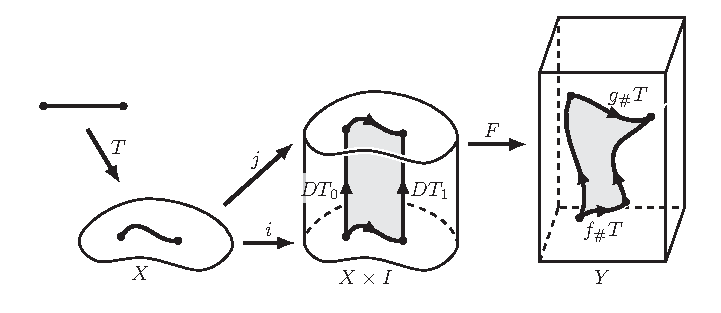
\includegraphics[width=.96\textwidth]{figures/4-3-1.pdf}\\图 4.3.1\end{center}
将 $D$ 的存在性单列为引理。

\entry{引理}{4.3.6}对每个空间 $X$ 及每个非负整数 $p$，存在同态
\[
D_X:S_p(X)\to S_{p+1}(X\times I),
\]
具有下列性质：
\begin{enumerate}[label=(\alph*)]
\item 对每个奇异单形 $T:\Delta_p\to X$，有 $\partial D_XT+D_X\partial T=j_\#T-i_\#T$，其中 $i(x)=(x,0)$、$j(x)=(x,1)$。
\item $D_X$ 具有自然性：若 $f:X\to Y$ 连续，则下图交换（$i_I$ 为 $I$ 的恒等映射）：
\[
\begin{array}{ccc}
S_p(X)&\xrightarrow{D_X}&S_{p+1}(X\times I)\\
\downarrow\scriptstyle f_\#&&\downarrow\scriptstyle(f\times i_I)_\#\\
S_p(Y)&\xrightarrow{D_Y}&S_{p+1}(Y\times I).
\end{array}
\]
\end{enumerate}

\sourcepage{199}
\textbf{证明：}对 $p$ 归纳。先设 $p=0$。给定 $T:\Delta_0\to X$，以 $x_0$ 表示 $T(\Delta_0)$，定义
\[
D_XT(t,0,0,\ldots)=(x_0,t)\qquad(0\le t\le1).
\]
〔回忆 $\Delta_1=\epsilon_0\epsilon_1$ 正是所有这种形式的点组成的线段。〕性质 (a)、(b) 易于验证。

现设 $p>0$，并假定对所有空间，在小于 $p$ 的维数上都已定义满足 (a)、(b) 的 $D_X$。先在特殊情形 $X=\Delta_p$、$T=i_p$ 下定义 $D_XT$，其中 $i_p$ 为 $\Delta_p$ 的恒等映射。这正是方法的核心：先处理一个称为“模型空间”的特殊空间，以及其上一个特殊奇异单形。

令 $\widehat i,\widehat j:\Delta_p\to\Delta_p\times I$ 分别将 $x$ 映到 $(x,0)$、$(x,1)$。定义 $\Delta_p\times I$ 上的奇异链
\[
c_p=\widehat j_\#(i_p)-\widehat i_\#(i_p)-D_{\Delta_p}(\partial i_p).
\]
因为 $i_p\in S_p(\Delta_p)$，而 $\partial i_p\in S_{p-1}(\Delta_p)$，归纳假设保证最后一项已有定义。再由归纳假设，
\begin{align*}
\partial c_p&=\partial\widehat j_\#(i_p)-\partial\widehat i_\#(i_p)-\partial D_{\Delta_p}(\partial i_p)\\
&=\widehat j_\#(\partial i_p)-\widehat i_\#(\partial i_p)
-\bigl[\widehat j_\#(\partial i_p)-\widehat i_\#(\partial i_p)-D_{\Delta_p}\partial\partial i_p\bigr]=0.
\end{align*}
空间 $\Delta_p\times I$ 为凸集，由定理 4.2.9 无环。所以可选 $S_{p+1}(\Delta_p\times I)$ 中一个边缘为 $c_p$ 的元素，记为 $D_{\Delta_p}(i_p)$。于是
\[
\partial D_{\Delta_p}(i_p)=\widehat j_\#(i_p)-\widehat i_\#(i_p)-D_{\Delta_p}(\partial i_p),
\]
即满足 (a)。

对任意空间 $X$ 和任意奇异单形 $T:\Delta_p\to X$，定义
\[
D_XT=(T\times i_I)_\#\bigl(D_{\Delta_p}i_p\bigr),
\]
并线性延拓。见图 4.3.2。直观地，$D_{\Delta_p}i_p$ 是填满棱柱 $\Delta_p\times I$ 的奇异 $(p+1)$ 维链，其边缘大致就是棱柱的边缘；$(T\times i_I)_\#$ 将这个链映到 $X\times I$。

验证 (a)，计算得
\begin{align*}
\partial D_XT&=(T\times i_I)_\#\partial D_{\Delta_p}i_p\\
&=(T\times i_I)_\#\bigl(\widehat j_\#i_p-\widehat i_\#i_p-D_{\Delta_p}\partial i_p\bigr)\\
&=j_\#T-i_\#T-(T\times i_I)_\#D_{\Delta_p}(\partial i_p).\tag{*}
\end{align*}
\sourcepage{200}
\begin{center}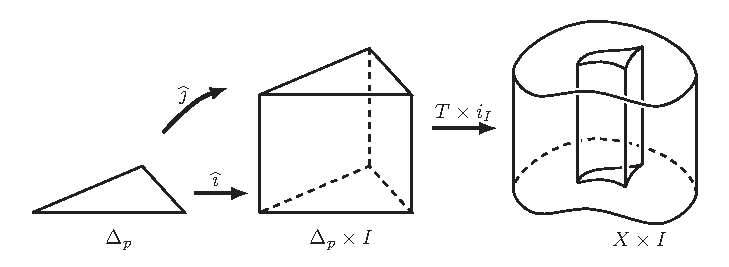
\includegraphics[width=.96\textwidth]{figures/4-3-2.pdf}\\图 4.3.2\end{center}
由低一维的自然性归纳假设，下图交换：
\[
\begin{array}{ccc}
S_{p-1}(\Delta_p)&\xrightarrow{D_{\Delta_p}}&S_p(\Delta_p\times I)\\
\downarrow\scriptstyle T_\#&&\downarrow\scriptstyle(T\times i_I)_\#\\
S_{p-1}(X)&\xrightarrow{D_X}&S_p(X\times I).
\end{array}
\]
故 $(T\times i_I)_\#D_{\Delta_p}(\partial i_p)=D_XT_\#(\partial i_p)=D_X\partial T$，式 (*) 正是所求。

验证 (b) 更为直接。若 $f:X\to Y$，则 $(f\circ T)\times i_I=(f\times i_I)\circ(T\times i_I)$。由定义，
\begin{align*}
D_Y(f_\#T)&=D_Y(f\circ T)=((f\circ T)\times i_I)_\#D_{\Delta_p}(i_p)\\
&=((f\times i_I)\circ(T\times i_I))_\#D_{\Delta_p}(i_p)=(f\times i_I)_\#D_XT.
\end{align*}

上述证明在 $p=0$ 时直接构造 $D_X$，只在归纳步骤中用了模型空间。下面给出一个更像归纳步骤的零维证明；后面将推广的正是这种证明。

先对 $X=\Delta_0$、$T=i_0$ 定义 $D_XT$。所需等式为
\[
\partial D_{\Delta_0}(i_0)=\widehat j_\#(i_0)-\widehat i_\#(i_0).
\]
右端是 $\Delta_0\times I$ 中增广为零的零维链。该空间为凸集，故无环；可选择一个一维链 $D_{\Delta_0}(i_0)$，使其边缘为右端。对于一般的 $X$ 和 $T$，令 $D_XT=(T\times i_I)_\#D_{\Delta_0}(i_0)$。性质 (a)、(b) 的证明与归纳步骤完全相同。\hfill$\square$

\sourcepage{201}
\entry{定理}{4.3.7}若 $f,g:(X,A)\to(Y,B)$ 同伦，则 $f_*=g_*$。当 $A=B=\varnothing$ 时，约化同调也有同样结论。

\textbf{证明：}设 $F:(X\times I,A\times I)\to(Y,B)$ 是从 $f$ 到 $g$ 的同伦，$i(x)=(x,0)$、$j(x)=(x,1)$。由 $D_X$ 对包含映射 $A\to X$ 的自然性，其在 $S_p(A)$ 上的限制为 $D_A$。所以 $D_X$ 将 $S_p(A)$ 映入 $S_{p+1}(A\times I)$，在相对链上诱导
\[
D_{X,A}:S_p(X,A)\to S_{p+1}(X\times I,A\times I),
\]
并满足引理 4.3.6(a) 的公式。令 $D=F_\#D_{X,A}$，其中
\[
F_\#:S_{p+1}(X\times I,A\times I)\to S_{p+1}(Y,B).
\]
于是
\begin{align*}
\partial D&=F_\#\partial D_{X,A}=F_\#(j_\#-i_\#-D_{X,A}\partial)\\
&=(F\circ j)_\#-(F\circ i)_\#-D\partial=g_\#-f_\#-D\partial.
\end{align*}
故 $f_\#$ 与 $g_\#$ 链同伦。\translatornote{原书最后一行写为 $f_\#-g_\#-D\partial$；若同伦按 $F(x,0)=f(x)$、$F(x,1)=g(x)$ 约定，则应如上。结论不受此符号笔误影响。}\hfill$\square$

\entry{定义}{4.3.8}设 $f:(X,A)\to(Y,B)$。若存在 $g:(Y,B)\to(X,A)$，使 $f\circ g$、$g\circ f$ 作为空间偶的映射分别同伦于相应恒等映射，则称 $f$ 为\textbf{同伦等价}，$g$ 为 $f$ 的\textbf{同伦逆}。

\entry{定理}{4.3.9}设 $f:(X,A)\to(Y,B)$。
\begin{enumerate}[label=(\alph*)]
\item 若 $f$ 为同伦等价，则 $f_*$ 在相对同调中为同构。
\item 更一般地，若 $f:X\to Y$ 与 $f|_A:A\to B$ 都是同伦等价，则 $f_*$ 在相对同调中为同构。
\end{enumerate}
\textbf{证明：}(a) 立即由同伦公理得到。证明 (b)，考察 $(X,A)$ 和 $(Y,B)$ 的长正合列及 $f_*$ 诱导的两列间同态。假设说明 $f_*:H_p(X)\to H_p(Y)$ 与 $(f|_A)_*:H_p(A)\to H_p(B)$ 都是同构。由 Steenrod 五引理（引理 3.3.4）即得结论。\hfill$\square$

\sourcepage{202}
若 $f:(X,A)\to(Y,B)$ 是同伦等价，则 $f:X\to Y$、$f|_A:A\to B$ 也都是同伦等价，反之却不成立，如下例所示。

\entry{例}{4.3.10}考虑包含映射 $j:(B^n,S^{n-1})\to(\R^n,\R^n\setminus\{0\})$。由于 $B^n$ 是 $\R^n$ 的形变收缩核，而 $S^{n-1}$ 是 $\R^n\setminus\{0\}$ 的形变收缩核，$j_*$ 在相对同调中为同构。

若存在 $j$ 的同伦逆 $g:(\R^n,\R^n\setminus\{0\})\to(B^n,S^{n-1})$，则因 $0$ 是 $\R^n\setminus\{0\}$ 的极限点，连续性迫使 $g(0)\in S^{n-1}$。所以 $g\circ j$ 将整个 $B^n$ 映入 $S^{n-1}$，在相对同调上诱导零同态。然而它按假设同伦于恒等映射，故在 $H_n(B^n,S^{n-1})$ 上诱导恒等同态。我们很快会证明此群非零，从而得到矛盾。

\subsection*{习题}
\begin{enumerate}
\item 构造奇异同调中三元组的正合列。〔见第 3.3 节习题 1 和第 3.5 节习题 2。〕
\item 证明：若 $f:X\to Y$ 同伦于常值映射，则 $f_*$ 在约化同调中为零同态。由此推出可缩空间的奇异同调无环。
\item 设包含映射 $j:A\to X$ 是同伦等价。证明 $H_p(X,A)=0$。
\item 举例说明：虽然 $X$ 与 $Y$ 同伦等价，$A$ 与 $B$ 同伦等价，仍可能有 $H_p(X,A)\not\cong H_p(Y,B)$。与定理 4.3.9 比较。
\item 引理 4.3.6 的证明中，选择链 $D_{\Delta_p}i_p$ 有一定自由。证明下式给出的 $\Delta_p\times I$ 中的 $(p+1)$ 维链满足该引理的要求：
\[
\begin{split}
D_{\Delta_p}i_p=\sum_{i=0}^p(-1)^i\ell\bigl(& (\epsilon_0,0),(\epsilon_1,0),\ldots,(\epsilon_i,0),\\
& (\epsilon_i,1),(\epsilon_{i+1},1),\ldots,(\epsilon_p,1)\bigr).
\end{split}
\]
\translatornote{原书求和中的系数印为 $(-1)^p$；棱柱链中各项应取交替符号 $(-1)^i$。}分别画出 $p=1$、$p=2$ 的图形。
\item 证明：若 $f:(X,A)\to(Y,B)$ 是同伦等价，则 $f:X\to Y$ 与 $f|_A:A\to B$ 都是同伦等价。
\item 考虑以链复形为对象的范畴 $\mathcal C$。从 $C$ 到 $C'$ 的 $d$ 次态射是同态族 $\varphi_p:C_p\to C'_{p+d}$。考虑从拓扑范畴到 $\mathcal C$ 的函子
\[
G(X)=\mathcal S(X),\quad G(f)=f_\#;\qquad
H(X)=\mathcal S(X\times I),\quad H(f)=(f\times i_I)_\#.
\]
证明引理 4.3.6 的链同伦是从 $G$ 到 $H$ 的自然变换。
\item 验证 $p=0$ 时，引理 4.3.6 的性质 (a)、(b) 成立。
\item 证明：若 $X$ 由 $n$ 个点组成，并赋予离散拓扑，则 $p\ne0$ 时 $H_p(X)=0$，且 $H_0(X)\cong\Z^n$。
\item 给出一个满足 $H_1(X)=\Z$ 的空间 $X$。
\item 给出一个满足 $H_1(Y)=\Z\times\Z$ 的空间 $Y$。
\end{enumerate}
